% Copyright (c)  2005-2010 EDF-EADS-PHIMECA.
% Permission is granted to copy, distribute and/or modify this document
% under the terms of the GNU Free Documentation License, Version 1.2
% or any later version published by the Free Software Foundation;
% with no Invariant Sections, no Front-Cover Texts, and no Back-Cover
% Texts.  A copy of the license is included in the section entitled "GNU
% Free Documentation License".
\renewcommand{\filename}{docUC_ThresholdExceedance_FORMExploitation.tex}
\renewcommand{\filetitle}{UC : Run and results exploitation  of a FORM/SORM algorithm : probability estimation, importance factors, reliability indexes, sensitivity factors}

% \HeaderNNIILevel
% \HeaderIILevel
\HeaderIIILevel

\index{Threshold Probability!SORM Breitung, Tvedt, Hohenbichler}
\index{Sensitivity Analysis!FORM probability}
\index{Sensitivity Analysis!Hasofer reliability index}
\index{Graph!FORM/SORM importance factors}
\index{Graph!Hasofer reliability index sensitivity}
\index{Graph Manipulation!ViewImage}
\index{Graph Manipulation!Show}



The objective of this Use Case is to launch the analytical algorithm and exploit all the associated results :
\begin{itemize}
\item the design point in both physical and standard space,
\item the probability estimation accoding to the FORM approximation, and the following SORM ones : Tvedt, Hohen-Bichler and Breitung,
\item the Hasofer reliability index and the generalized ones evaluated from the Breitung, Tvedt and Hohen-Bichler approximations,
\item the \emph{classical} importance factors defined as the normalized director factors of the design point in the $\bdU$-space  :
  \begin{equation}\label{def1}
    \alpha_i^2 = \displaystyle \frac{(u_i^{*})^2}{\beta_{HL}^2}
  \end{equation}
  if we note $\vect{u}^*$ the design point in the $\bdU$-space. These importance factors are accessible with the methods \emph{getImportanceFactors(True)} or  \emph{drawImportanceFactors(True)} where the boolean $True$ specifies the formula (\ref{def1});
\item the \emph{innovative} importance factors defined in (\ref{def2}) in the elliptical space of  the iso-probabilistic transformation, where the marginal distributions are all elliptical, with  cumulative distribution function noted $E$, and not yet decorrelated.\\
In the case where the input distribution of $\vect{X}$ has an elliptical copula $C_E$, then $E$ has the same type as  $C_E$.\\
In the case where the input distribution of $\vect{X}$ has a copula $C$ which is not elliptical, then  $E=\Phi$ where $\Phi$ is the CDF of the standard normal.\\ 
This innovative definition of importance factors has the advantage to be one-to-one between the $X_i$ components and the $Y_i$ ones :
  \begin{equation}\label{def2}
    \alpha_i^2 = \displaystyle \frac{(y_i^{*})^2}{||\vect{y}^{*}||^2}
  \end{equation}
where 
  \begin{eqnarray}
    \boldsymbol{Y}^* =  \left(
      \begin{array}{c}
        E^{-1}\circ F_1(X_1^*) \\
        E^{-1}\circ F_2(X_2^*) \\
        \vdots \\
        E^{-1}\circ F_n(X_n^*)
      \end{array}
    \right).\label{varY10}
  \end{eqnarray}
whith $\vect{X}^*$ is the design point in the physical space. If not specified, the importance factors are evaluated from (\ref{def2}).\\
Note that (\ref{def1}) and  (\ref{def2}) coïncide in the case of independent components $X_i$.

\item the sensitivity factors of the Hasofer reliability index and the FORM probability.
\item the coordinates of the mean point in the standard event space :  $\displaystyle \frac{1}{E_1(-\beta)}\int_{\beta}^{\infty} u_1 p_1(u_1)du_1$ where $E_1$ is the spheric univariate distribution of the standard space and $\beta$ the reliability index.
\end{itemize}



Details on FORM algorithm  may be found in the Reference Guide (\href{OpenTURNS_ReferenceGuide.pdf}{see files Reference Guide - Step C -- FORM and  - Step Cp -- Importance Factors from FORM-SORM methods}).\\


Details on each object may be found in the User Manual  (\href{OpenTURNS_UserManual_TUI.pdf}{see User Manual - Threshold exceedance probability evaluation with reliability algorithm / Reliability Algorithms}).\\


Warning! Check the quality of your gradient and hessian implementations as the SORM approximation relies on an accurate computation of the main curvatures of the limit state function at the design point, which needs an accurate evaluation of both the gradient and the hessian at this point. \\


\requirements{
  \begin{description}
  \item[$\bullet$] the analytical algorithm : {\itshape myAlgo}
  \item[type:] FORM or SORM
  \item[$\bullet$] the limit state function {\itshape limitStateFunction} such as : {\itshape output = limitStateFunction(input)}
  \item[type:] NumericalMathFunction
  \end{description}
}
{
  \begin{description}
  \item[$\bullet$] SORM Event probabilities (Breitung, HohenBichler and Tvedt approximations)
  \item[type:] NumericalScalar
  \item[$\bullet$] Reliability Index
  \item[type:] NumericalScalar
  \item[$\bullet$] Importance factors
  \item[type:] NumericalPoint
  \item[$\bullet$] Reliability index Sensitivity factors
  \item[type:] AnalyticalSensitivity
  \item[$\bullet$] Mean point in event standard space
  \item[type:] NuemricalPoint
  \item[$\bullet$] graphs
  \item[type:] Graph
  \end{description}
}

\textspace\\



\begin{lstlisting}
  # Save the number of calls to the limit state fucntion, its gradient and hessian already done
  limitStateFunctionCallNumberBefore = limitStateFunction.getEvaluationCallsNumber()
  limitStateFunctionGradientCallNumberBefore = limitStateFunction.getGradientCallsNumber()
  limitStateFunctionHessianCallNumberBefore = limitStateFunction.getHessianCallsNumber()

  # Perform the simulation
  myAlgo.run()

  # Save the number of calls to the limit state fucntion, its gradient and hessian already done
  limitStateFunctionCallNumberAfter = limitStateFunction.getEvaluationCallsNumber()
  limitStateFunctionGradientCallNumberAfter = limitStateFunction.getGradientCallsNumber()
  limitStateFunctionHessianCallNumberAfter = limitStateFunction.getHessianCallsNumber()

  # Display the number of iterations executed and
  # the number of evaluations of the limit state function
  print "number of evaluations of the limit state function = ",
  limitStateFunctionCallNumberAfter - limitStateFunctionCallNumberBefore

  # Stream out the result
  result = myAlgo.getResult()

  # Hasofer reliability index
  print  "Hasofer reliability index=" , result.getHasoferReliabilityIndex()

  # Generalized reliability index
  # FORM study : generalized reliability index is the Hasofer one
  print  "generalized reliability index=" , result.getGeneralisedReliabilityIndex()

  # SORM study
  # with Breitung approximation
  print  "Breitung generalized reliability index=", result.getGeneralisedReliabilityIndexBreitung()

  # with  HohenBichler approximation
  print  "HohenBichler generalized reliability index=", result.getGeneralisedReliabilityIndexHohenBichler()

  # with Tvedt approximation
  print  "Tvedt generalized reliability index=", result.getGeneralisedReliabilityIndexTvedt()

  # Design point in the standard and physical spaces
  print  "standard space design point=" , result.getStandardSpaceDesignPoint()
  print  "physical space design point=" , result.getPhysicalSpaceDesignPoint()

  # Is the standard point origin in failure space?
  print "is standard point origin in failure space? ", result.getIsStandardPointOriginInFailureSpace()

  # FORM probability of the event
  print  "event probability=" , result.getEventProbability()

  # SORM probability of the event
  # with Breitung approximation
  print  "Breitung event probability=", result.getEventProbabilityBreitung()

  # with  HohenBichler approximation
  print  "HohenBichler event probability=", result.getEventProbabilityHohenBichler()

  # with Tvedt approximation
  print  "Tvedt event probability=", result.getEventProbabilityTvedt()

  # Get the mean point in standard event space
  print "Mean point in standard event space= ", result.getMeanPointInStandardEventDomain()

  # Importance factors : numerical results
  # Y-space definition
  print  "importance factors=" , result.getImportanceFactors()
  # U-space definition
  print  "importance factors=" , result.getImportanceFactors(True)

  # GRAPH 1 : Importance Factors graph
  # Y-space definition
  importanceFactorsGraph = result.drawImportanceFactors()
  # U-space definition
  importanceFactorsGraph = result.drawImportanceFactors(True)

  importanceFactorsGraph.draw("ImportanceFactorsDrawingFORM")

  # View the bitmap file
  ViewImage(importanceFactorsGraph.getBitmap())

  # Check that the correct files have been generated
  # by computing their checksum
  print "bitmap=" , importanceFactorsGraph.getBitmap()
  print "postscript=" , importanceFactorsGraph.getPostscript()

  # In order to see the graph without creating the associated files
  Show(importanceFactorsGraph)

  # Hasofer Reliability Index Sensitivity : numerical results
  hasoferReliabilityIndexSensitivity = result.getHasoferReliabilityIndexSensitivity()
  print "hasoferReliabilityIndexSensitivity = " , hasoferReliabilityIndexSensitivity

  # GRAPH 2 : Hasofer Reliability Index Sensitivity Graphs
  reliabilityIndexSensitivityGraphs = result.drawHasoferReliabilityIndexSensitivity()

  # Sensitivity to parameters of the marginals of
  # the input random vector
  graph2a = reliabilityIndexSensitivityGraphs[0]
  graph2a.draw("HasoferReliabilityIndexMarginalSensitivityDrawing")

  # View the bitmap file
  ViewImage(graph2a.getBitmap())

  # Check that the correct files have been generated
  # by computing their checksum
  print "bitmap=" , graph2a.getBitmap()
  print "postscript=" , graph2a.getPostscript()

  # In order to see the graph without creating the associated files
  Show(graph2a)

  # Sensitivity to the other parameters (dependance)
  graph2b = reliabilityIndexSensitivityGraphs[1]
  graph2b.draw("HasoferReliabilityIndexOtherSensitivityDrawing")

  # or in order to quickly draw it : with default options
  # default options : 640, 480 and the files are on the current repertory
  importanceFactorsGraph.draw("ImportanceFactorsDrawingFORM")
  # View the bitmap file
  ViewImage(graph2b.getBitmap())

  # Check that the correct files have been generated
  # by computing their checksum
  print "bitmap=" , graph2b.getBitmap()
  print "postscript=" , graph2b.getPostscript()

  # In order to see the graph without creating the associated files
  Show(graph2b)

  # FORM Event Probability Sensitivity : numerical results
  eventProbabilitySensitivity = result.getEventProbabilitySensitivity()
  print "eventProbabilitySensitivity = " , eventProbabilitySensitivity

  # GRAPH 3 : FORM Event Probability Sensitivity Graphs
  eventProbabilitySensitivityGraphs = result.drawEventProbabilitySensitivity()

  # Sensitivity to parameters of the marginals of the input random vector
  graph3a = eventProbabilitySensitivityGraphs[0]
  graph3a.draw("EventProbabilityIndexMarginalSensitivityDrawing")

  # View the bitmap file
  ViewImage(graph3a.getBitmap())

  # Check that the correct files have been generated
  # by computing their checksum
  print "bitmap=" , graph3a.getBitmap()
  print "postscript=" , graph3a.getPostscript()

  # In order to see the graph without creating the associated files
  Show(graph3a)

  # Sensitivity to the other parameters (dependance)
  graph3b = eventProbabilitySensitivityGraphs[1]
  graph3b.draw("EventProbabilityIndexOtherSensitivityDrawing")

  # View the bitmap file
  ViewImage(graph3b.getBitmap())

  # Check that the correct files have been generated
  # by computing their checksum
  print "bitmap=" , graph3b.getBitmap()
  print "postscript=" , graph3b.getPostscript()

  # In order to see the graph without creating the associated files
  Show(graph3b)
\end{lstlisting}
\textspace\\


Figure \ref{FORMImportanceFactors}  shows an importance factors pie evaluated from the FORM method, in the beam example described in Eq. (\ref{equatPoutre}), where :
\begin{itemize}
\item $E$ follows the Beta($r = 0.94$, $t = 3.19$, $a = 2.78e7$, $b = 4.83e7$) distribution,
\item $F$ follows the LogNormal($\mu = 3e5$, $\sigma = 9e3$, $\gamma = 1.5e4$)  distribution,
\item $L$ follows the Uniform($a = 250$, $b=260$) distribution,
\item $I$ follows the Beta($r = 2.5$, $t = 4.0$, $a = 3.1e2$, $b = 4.5e2$) distribution,
\item the four components are independant.
\end{itemize}

The output is expressed in centimeters.\\
The event considered is :
$$
myEvent = \{ output=f(input) \leq -30 \}.
$$
\begin{figure}[H]
  \begin{center}
    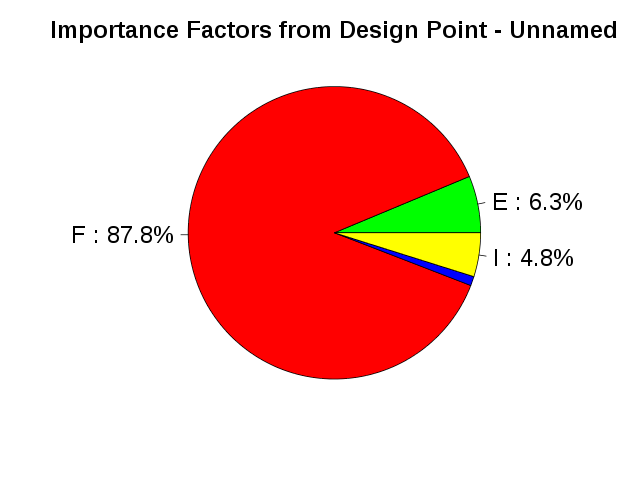
\includegraphics[width=10cm]{ImportanceFactorsDrawingFORM.png}
  \end{center}
  \caption{Importance factors from the FORM method.}
  \label{FORMImportanceFactors}
\end{figure}

\begin{figure}[H]
  \begin{center}
    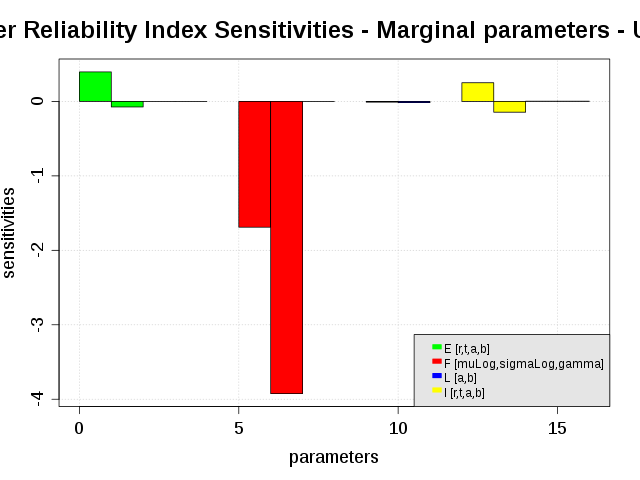
\includegraphics[width=10cm]{HasoferReliabilityIndexMarginalSensitivityDrawing.png}
  \end{center}
  \caption{Hasofer Reliability Index sensitivities with respect to the marginal parameters.}
  \label{FORMIndexSensitivity}
\end{figure}

\begin{figure}[H]
  \begin{center}
    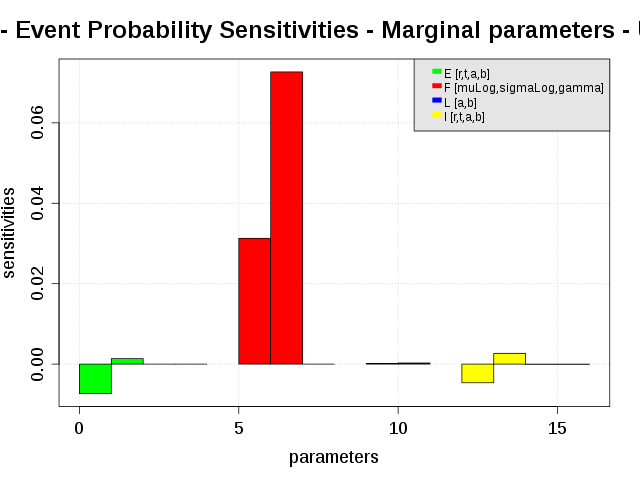
\includegraphics[width=10cm]{EventProbabilityIndexMarginalSensitivityDrawing.png}
  \end{center}
  \caption{FORM probability sensitivities with respect to the marginal parameters.}
  \label{FORMProbaSensitivity}
\end{figure}
